%\documentclass[11pt,notoc,nolof,nolot,nomaketitle,combinedbib]{combine}
\documentclass[12pt]{article}

\usepackage{amsmath}
\usepackage{graphicx}
\usepackage{amsfonts}
\usepackage{amsthm}
%\usepackage{cite}
\usepackage{times}
\usepackage{geometry}
\usepackage[round,numbers,sort&compress]{natbib}
\oddsidemargin=0.0in %%this makes the odd side margin go to the default of 1inch
\evensidemargin=0.0in
\textwidth=6.5in
\textheight=9in %%sets the textwidth to 6.5, which leaves 1 for the remaining right margin with 8 1/2X11inch paper

\providecommand{\ve}[1]{\vec{#1}}
\providecommand{\ma}[1]{\boldsymbol{#1}}
\providecommand{\norm}[1]{\left \lVert#1 \right  \rVert}
%\providecommand{\Ltwo}[1]{\left \lVert#1 \right  \rVert_2^2}
\providecommand{\deter}[1]{\lvert #1 \rvert}
\providecommand{\abs}[1]{\lvert #1 \rvert}
\providecommand{\tran}{\mbox{${}^{\text{T}}$}}
\providecommand{\transpose}{\mbox{${}^{\text{T}}$}}
\providecommand{\ve}[1]{\boldsymbol{#1}}
\DeclareMathOperator*{\argmax}{argmax}
\DeclareMathOperator*{\argmin}{argmin}
\DeclareMathOperator*{\find}{find}

\newcommand{\Lik}{\mathcal{L}}
\newcommand{\Ca}{[\text{Ca}^{2+}]}
\newcommand{\Cae}{[\widehat{\text{Ca}}^{2+}]}
\newcommand{\Cav}{\ve{C}}%[\ve{\text{Ca}}^{2+}]}
\newcommand{\sml}{\sqrt{\ma{\lambda}}}
\newcommand{\ml}{\ma{\lambda}}

\newcommand{\nw}{\widehat{n}}
\newcommand{\nv}{\vec{n}}

\newcommand{\Ae}{\widehat{A}}
\newcommand{\te}{\widehat{\tau}}
%\newcommand{\A}{\widehat{A}^{(i)}}
%\newcommand{\t}{\widehat{\tau}^{(i)}}
%\newcommand{\s}{\widehat{\sigma}^{(i)}}
%\newcommand{\B}{\widehat{B}^{(i)}}

%\usepackage[hypertex]{hyperref}    %for LaTeX
\usepackage{hyperref}               %for pdfLaTeX

\title{Fast Methods Comp}

\author{Joshua T. Vogelstein%\footnote{Corresponding author: joshuav@jhu.edu}
, Baktash Babadi, Liam Paninski
%$\,$ and Liam Paninski$^\#$ \\ $^\ast$ Department of Neuroscience, Johns Hopkins School of Medicine \\ $^\#$ Department of Statistics and Center for Theoretical Neuroscience, Columbia University
}

\begin{document}
\maketitle %\pagenumbering{roman}
%\setcounter{secnumdepth}{0}
%\pagenumbering{roman} %\setcounter{page}{-10}
%\pagestyle{headings}
\tableofcontents
%\listoffigures
%\listoftables

\begin{abstract}

\end{abstract}

\section{Introduction}

The goal of this work is to infer the underlying spike train, having only the observed fluorescence signal available to us.  To do so, we propose a parametric model of the experimental system.  Then, we develop a number of algorithms, each iteratively estimating the parameters and then using those parameters to infer the hidden spike trains.  

\section{Methods}
\subsection{Model}

First, for simplicity, we assume that we have extracted a time series of fluorescence observations, $F_t$, which is a function of the intracellular calcium concentration of the imaged soma at that time, $\Ca_t$.  In particular, we assume that $F_t$ simply a noisy version of $\Ca_t$, i.e.,

\begin{align} \label{eq:F}
F_t &=  \Ca_t + \varepsilon_t, \qquad \varepsilon_t \sim \mathcal{N}(0,\sigma^2)
\end{align}

\noindent where $\varepsilon_t$ is an additive Gaussian noise term with zero mean and variance $\sigma^2$. Note that this time series is naturally discrete, with time step size $\Delta$ corresponding to the frame rate of the image acquisition system, with $t$ indexing the time step, and $T$ indicating the final time step. The $\Ca$ signal is assumed to jump immediate after each spike by $A$ $\mu$M and then decay back to rest, $\Ca_0$, with time constant $\tau$ sec.  Therefore, we have:

\begin{align} \label{eq:C}
\Ca_t = a \Ca_{t-1} +  A n_t + b,
\end{align}

\noindent where we have parameters $a=1-\frac{\Delta}{\tau}$ and $b=\frac{\Delta}{\tau}\Ca_0$, where $\Ca_0$ is the baseline $\Ca$, and $n_t$ is the underlying spike train. Figure \ref{fig:comp} shows an example fluorescence time-series (A), the true calcium signal (B), and the true spike train (C).

\subsection{Inferring the spike times}

There are a number of ways one could go about inferring the hidden spike train from the fluorescence time series.  Below, we develop a number of Bayesian approaches, in which we first define a likelihood that we would like to maximize, and then propose an efficient algorithm for maximizing that likelihood.

\paragraph{Least-Squares Solution}

We would like to find the most likely spike train that led to the observed fluorescence signal. This problem may be formally cast as finding a spike train that maximizes the likelihood of the fluorescence observations.  As the only source of noise is the $\varepsilon_t$ on the observations, which is Gaussian, we have: 

\begin{align} \label{eq:lsq}
\ve{n}_{lsq} &= \argmax_{\ve{n}} \sum_{t=0}^T \varepsilon_t^2\\
&= \argmax_{\ve{n}} \sum_{t=0}^T \frac{1}{2\sigma^2}\exp\left\{-\frac{1}{2}\left(\frac{F_t-\Ca_t}{\sigma}\right)^2\right\}\\
&= \argmin_{\ve{n}} \sum_{t=0}^T (F_t - \Ca_t)^2
\end{align}

\noindent where we use the notation $\ve{n}=n_0,\ldots, n_T$, and $\Ca$ is implicitly a function of $n$.  As \eqref{eq:lsq} is a quadratic optimization problem, it may be solved with any gradient ascent technique.  In particular, for any quadratic problem:

\begin{align} \label{eq:lsq0}
\ve{x}_{lsq} = \argmin_{\ve{x}} \norm{\ma{Y} \ve{x} - \ve{z}}_2^2,
\end{align}

\noindent the analytical solution is simply:

\begin{align}
\ve{x}_{lsq} = \ve{x}_0 - (\ma{Y}'\ma{Y})^{-1} \ma{Y}'\ve{z} 
= \ve{x}_0-\ma{H}^{-1}\ve{g}
\end{align}

\noindent where $\ve{x}_0$ is some initial guess for the value of $\ve{x}$, $\ma{H}$ is the Hessian matrix (i.e., second derivative of $\norm{\ma{Y} \ve{x} + \ve{z}}_2^2$ with respect to $\ve{x}$, and $\ve{g}$ is the gradient vector (i.e., first  derivative of $\norm{\ma{Y} \ve{x} + \ve{z}}_2^2$ with respect to $\ve{x}$. Thus to solve any quadratic optimization problem, one must simply cast it in the form of \eqref{eq:lsq0} and then solve for $\ma{H}$ and $\ve{h}$. The key to solving \eqref{eq:lsq} problem efficiently is to write $\ve{n}$ as a function of $\Cav=[\Ca_0,\ldots,\Ca_T]$. In particular, after subtracting $b$, we may write:

\begin{align} \label{eq:nMC}
\ve{n}=\ma{M}\Cav
\end{align}

\noindent where $\ma{M}$ is a $T \times T$ bidiagonal deconvolution matrix:

\begin{equation} \label{eq:M}
\ma{M}=\begin{bmatrix}
1/A&0&0&0&\ldots&0\\
-a/A&1/A&0&0&\ldots&0\\
0&-a/A&1/A&0&\ldots&0\\
\vdots\\
0&\ldots&0&0&-a/A&1/A
\end{bmatrix}.
\end{equation}

\noindent which follows from \eqref{eq:C}. Thus, letting $c=1/(2\sigma^2)$ we may rewrite \eqref{eq:lsq}, and solve for $\ve{g}$ and $\ma{H}$:

\begin{align}
\Cav_{lsq} &= \argmin_{\Cav} c\norm{\ve{F}-\Cav}_2^2\\
\ve{g} &= -2c(\ve{F}-\Cav)\\
\ma{H}&= 2c\ma{I}
\end{align}

\noindent where $\ma{I}$ is an identity matrix of appropriate size.  Thus,

\begin{align}
\Cav_{lsq} = \Cav-(2\ma{I})^{-1} \big(-2c(\ve{F}-\Cav)\big)=\ve{F},
\end{align}

\noindent and therefore, $\ve{n}_{lsq}=\ma{M}\ve{F}$.
%Because the likelihood $\Lik$ of $\ve{n}_{\eta}$ is log-concave, we can use the Newton approach, which requires computing the gradient $\ve{g}$ and Hessian $\ma{H}$, and stepping in the direction of $\ma{H}^{-1}\ve{g}$.  
%Because $\ma{M}$ is bidiagonal, $\ma{H}$ is tridiagonal, so this computation may be performed in $O(T)$ time instead of the typical $O(T^3)$ time required for matrix inversions. 
%(details for efficiently computing the necessary terms may be found in Appendix \ref{sec:bar}).  Figure \ref{fig:comp}(D) shows why the solution to \eqref{eq:lsq} is problematic. 
This solution, plotted in Figure \ref{fig:comp}(D), is problematic for several reasons. First, in periods of quiescence (i.e., no spiking), the algorithm incorrectly infers the presence of many ``spikelets'', which do not exist in the true data.  Second, the algorithm sometimes infers \emph{negative} spikes, which also cannot exist. Third, the number of spikes in a frame is not necessarily an integer.  Each of these issues may be treated using standard tools from the optimization literature.

\paragraph{Regularizing}

To deal with the spikelets, we use a technique called ``regularizing''.  Essentially, we impose a prior on the probability of their being a spike at any time, and then we penalize the solution if it infers too many spikes.  Formally, we write:

\begin{align} \label{eq:reg}
\ve{n}_{reg} &= \argmin_{\ve{n}} \sum_{t=0}^T c \big((F_t - \Ca_t)^2 + f_{reg}(n_t) \big),
\end{align}

\noindent where $f_{reg}(n_t)$ is some regularizing function of $n_t$, typically chosen such that the likelihood remains concave.  For example, $f_{reg}(n_t)=\lambda_t n_t^2$, where $\lambda_t=1/($expected $n_t$), then we have a standard \emph{smoothing prior}.\footnote{This may be thought of as a generalization of ridge regression and Wiener deconvolution.}  To solve \eqref{eq:reg} efficiently with a smoothing prior, we rewrite \eqref{eq:reg} as a function of $\Cav$:

\begin{align} \label{eq:reg2}
\Cav_{reg} &= \argmin_{\Cav} c\norm{\ve{F}-\Cav}_2^2 + \norm{\sml\ma{M}\Cav}_2^2
\end{align}


\noindent where $\sml$ is a matrix with components $\sqrt{\lambda_t}$ along the diagonal and zeros elsewhere. Because this is also a quadratic problem, the solution is given by finding Hessian and gradient with respect to $\Cav$:

\begin{align}
\ve{g} &= -2c(\ve{F}-\Cav)+2 (\sml\ma{M}\Cav)'(\sml\ma{M})\\
\ma{H} &= 2c\ma{I}+2(\sml\ma{M})'(\sml\ma{M})
\end{align}

The key to solving this problem efficiently is that the Hessian is a tridiagonal matrix (which follows from the fact that $\sml$ is diagonal and $\ma{M}$ is bidiagonal).  Therefore, $\ma{H}^{-1}\ve{g}$ may be solved in $O(T)$ time (for instance, using Matlab's $\backslash$), instead of the typical $O(T^3)$ time normally required.  Figure \ref{fig:comp}(F) shows the results of \eqref{eq:reg2}.  Problematically, the solutions from such an approach possibly yield negative spikes, which are not possible in the true spike train.  

\paragraph{Barrier method}

It is of interest, therefore, to find the best underlying \emph{non-negative} spike train:

%$\lambda_t$ is the expected number of spikes at any time, and $n_t$ is squared because we want to penalize for any nonzero $n_t$ in such a way that conserves the concavity of optimization problem (i.e., so the unique solution can be found using any standard gradient search technique)\ref{??}.  Given a model of the neuron, the expected number of spikes could be a function of some external stimulus or spike histories, for example\ref{??}.  Otherwise, this parameter may simply be a guess as to the number of spikes the neuron likely emitted while imaging.  In either case, the effect of this regularizing term is to reduce the number of spikelets.  It comes at a cost, however, of reducing the size of the true spikes as well (see Figure \ref{fig:comp} D). It is worth noting here that $\ve{n}_{reg}$ is similar to the solution posed by Yaksi and Friedrich (2006)\ref{??}.

%While this regularizing term helps to deal with the spikelet problem, it does not solve the negative spikes problem. That problem may be solved by explicitly imposing a non-negativity constraint on the solution:

\begin{align} \label{eq:nng}
\ve{n}_{nng} &= \argmin_{\ve{n}: n_t \geq 0} \sum_{t=0}^T \big(c(F_t - \Ca_t)^2 +  \lambda_t n_t\big).
\end{align}

\noindent Note that we have chosen to let $f_{reg}(n_t)=\lambda n_t$ here, which ensures that not too many spikes are inferred. To efficiently solve this problem, we adopt the ``barrier method''.  This approach iteratively solves a related problem that penalizes the algorithm for inferring negative values, but with each iteration, reduces the penalty, in such a way that is guaranteed to converge to \eqref{eq:nng}\ref{??}.  Formally, it may be written as

\begin{align} \label{eq:b}
\ve{n}_{\eta} &= \argmin_{\ve{n}} \sum_{t=0}^T \big(c(F_t - \Ca_t)^2  + \lambda_t n_t + \eta f(n_t)\big),
\end{align}

\noindent where $f(n_t)$ is a barrier function, which is any function that approaches infinity from the right as $n_t$ approaches zero, e.g., $-\log(n_t)$.  So, as $\eta \rightarrow 0$, $\ve{n}_{\eta} \rightarrow \ve{n}_{nng}$. While this function is no longer quadratic, it is still concave. Therefore, the solution may be found be iterating any gradient descent technique.  The solution to Newton's method (which we used for both \eqref{eq:lsq} and \eqref{eq:reg}), in terms of $\Cav$, is:

\begin{align} \label{eq:newton}
\Cav_i = \Cav_{i-1} + s \ve{d}
\end{align}

\noindent where $s$ is the step size and $\ve{d}=\ma{H}^{-1}\ve{g}$ is the step direction.  $s$ must be chosen such that all of our constraints, namely $n_t>0$ for all $t$, are satisfied:

\begin{align}
0&< n_t\\
&< \ma{M}(\ve{C} + s \ve{d})\\
&< \ma{M} \ve{C} + s \ma{M} \ve{d}\\
\Rightarrow s &> -\ma{M}\ve{C} (\ma{M} \ve{d})^{-1}. \label{eq:s}
\end{align}

So $s$ must be larger than every component of the vector on the right-hand-side of the last inequality.  Furthermore, it is possible to ''over-step'', or rather, take a step so large as to \emph{increase} the likelihood that we are trying to minimize.  As such, prior to stepping, we check that the likelihood would indeed decrease, if not, we reduce $s$ until it does. 

To compute $\ve{d}$, we must solve for the Hessian and gradient of our likelihood function with respect to $\Cav$:

\begin{align}
\Cav_{est} &= \argmin_{\Cav} c \norm{\ve{F}-\Cav}_2^2 +\ml \ma{M}\Cav - \eta \log (\ma{M}\Cav)\\
\ve{g} &=-2c(\ve{F}-\Cav)+\ve{\lambda}\ma{M} - \eta \ma{M}' (\ma{M}\Cav)^{-1} \label{eq:bar_g}\\
\ma{H} &=2c\ma{I} + 2 \eta \ma{M}' (\ma{M}\Cav)^{-2}\ma{M} \label{eq:bar_H}.
\end{align}

Plugging $\ve{g}$ and $\ma{H}$ into \eqref{eq:newton} and then choosing the step size $s$ to satisfy \eqref{eq:s} and decrease the likelihood yields $\Cav_i$. This is iterated until it converges, at which time $\eta$ is reduced and the whole process repeats. Importantly, as for the regularized solution, the Hessian here is tridiagonal, facilitating $O(T)$ time to solve each Newton step, as opposed to $O(T^3)$, which would be unacceptably long for large data sets.  Pseudocode for an efficient implementation of this approach is provided in Table \ref{tab:bar}.  Figure \ref{fig:comp}(F) shows how this constraint further improves the inference accuracy.

\begin{table}[ht]
\caption{Pseudocode for barrier method}
\label{tab:bar}
\fbox{\begin{minipage}{1.0\linewidth}
For each $\eta$, let $\Cav_i$ be the current estimate of $\Cav$ (which may be initialized at $\ve{1}$ for instance).  While $\Cav_i < \Cav_{i-1}+\xi$ (for some small $\xi$), iterate the following steps.  When complete, reduce $\eta$ and repeat.
\begin{itemize}
\item Compute $\ve{g}$ using \eqref{eq:bar_g}
\item Compute $\ma{H}$ using \eqref{eq:bar_H}
\item Compute $\ve{d}=\ma{H}^{-1}\ve{g}$ efficiently
\item Choose $s$ such that \eqref{eq:s} is satisfied and the likelihood decreases upon plugging $s$ and $\ve{d}$ into \eqref{eq:newton}
\end{itemize}
\end{minipage}}
\end{table}

 %Because of the barrier method's qualitative and quantitative improvement over the least-squares or regularized formulations, \eqref{eq:lsq} and \eqref{eq:reg}, respectively, we do not consider them further.  

\paragraph{Projection Pursuit Regression (PPR)}

Although the barrier method provides us with a meaningful spike train inference, we can further constrain the inferred spike train to be integers, i.e.,

\begin{align} \label{eq:ppr}
\ve{n}_{ppr} &= \argmin_{\ve{n}: n_t \in 0,1,2,\ldots} \sum_{t=0}^T \big(c(F_t - \Ca_t)^2  + \lambda_t n_t\big).
\end{align}

\noindent Note that this formulation obviates the need to impose a non-negative constraint, but the prior  $\lambda_t n_t$ still performs a useful function.  In particular, in noisy scenarios, it helps the algorithm not infer too many spikes.  Pseudocode for an algorithm called \emph{projection pursuit regression} (PPR)\ref{FS81} which efficiently solving \eqref{eq:ppr} is provided in Table \ref{tab:ppr} .  Figure \ref{fig:comp}(G) shows the inferred spike train using this algorithm. Although this approach imposes a desirable constraint (i.e., that spike trains include only integers), it also comes at a cost relative to the barrier method, as will be described in Section \ref{sec:results}.

\begin{table}[h]
\caption{Pseudocode for PPR}
\label{tab:ppr}
\fbox{\begin{minipage}{1.0\linewidth}
This algorithm iterates several steps, as schematized by Figure \ref{fig:ppr_schem}. The algorithm is initialized with the fluorescence signal, which is the residual before iterating the following steps, $\ve{r}_0$:
\begin{itemize}
\item Compute the cross-correlation between the residual and the calcium kernel, 
\mbox{$xc(t)= r_i(t) \otimes A e^{-t/\tau}$}.
\item Let $t_{i+1}$ be the maximum of that cross-correlation,
\mbox{$t_{i+1} = \max_t xc(t)$}.
\item Let $\ve{o}_{i+1}$ be a zero vector with unity at $t_{i+1}$.  Convolve $\ve{o}_{i+1}$ with the calcium kernel to generate the $\Ca$ that would result from a spike having occurred at that time step,
\mbox{$\Ca_{i+1}(t) =  o_{i+1}(t) \ast A e^{-t/\tau}$}.
\item Subtract $[\ve{\text{Ca}}^{2+}]_{i+1}$ from the residual of the previous step to get the new residual,
\mbox{$\ve{r}_{i+1} = \ve{r}_i -  [\ve{\text{Ca}}^{2+}]_{i+1}$}.
\item Compute the sum of residual error, where $\ve{n}_{i+1}$ is a vector of zeros with ones inferred spike time,
\mbox{$\epsilon_{i+1} = \sum_t r_{i+1}(t)^2 + \lambda_t n_{i+1}(t)$}.
\item If $\epsilon_{i+1} < \epsilon_i$, repeat.  Otherwise, let $\ve{n}_{ppr} = \ve{n}_i$.
\end{itemize}
\end{minipage}}
\end{table}


\subsection{Inferring the parameters}

All of the above approaches assuming a particular effect of spikes on $\Ca$.  More precisely, they all assume that after each spike, $\Ca$ jumps by $A$ $\mu$M and then decays back to $\Ca_0$ $\mu$M with time constant $\tau$ sec.  Let $\Cae_t$ and $\widehat{n}_t$ be the estimated $\Ca_t$ and $n_t$, respectively.  We may then solve for:

\begin{align}
\{\widehat{a}, \widehat{A}, \widehat{b}\} &= \argmin_{a,A,b>0} \big(F_t - a \Cae_{t-1} - A \widehat{n}_t - b\big)^2.
\end{align}

\noindent where, as before, we have $a=1-\frac{\Delta}{\tau}$ and $b=\frac{\Delta}{\tau}\Ca_0$. This may be solved in matrix form by making the following substitutions:

\begin{align}
\Cav_{est} =\begin{bmatrix} \Cae_2\\ \vdots \\ \Cae_T \end{bmatrix},
\ve{n}_{est}=\begin{bmatrix} \widehat{n}_1\\ \vdots \\ \widehat{n}_{T-1} \end{bmatrix},
\ve{F}=\begin{bmatrix} F_1\\ \vdots \\ F_{T-1} \end{bmatrix},
\ma{G}=-\begin{bmatrix} \Cav_{est}\\ \ve{n}_{est}\\ \ve{1} \end{bmatrix}',
\quad \ve{x}=\begin{bmatrix} a\\ A\\ b \end{bmatrix},
\end{align}

\noindent where $\ve{1}$ is a column vector of ones of the appropriate length.  Thus, we may write another quadratic optimization problem:

\begin{align}
\ve{x}_{est}&=\argmin_{\ve{x}>\ve{0}} \frac{1}{T}\norm{\ma{D} \ve{x} + \ve{F}}_2^2\\
&=\argmin_{\ve{x}>\ve{0}} \frac{1}{T} (\ve{x}' \ma{D}'\ma{D} \ve{x} + 2 \ma{D}'\ve{F} \ve{x}
\end{align}

\noindent which may be efficiently solved using, for instance, Matlab's \texttt{quadprog}, plugging in $\ma{D}'\ma{D}$ for the quadratic term and $\ma{D}'\ve{F}$ for the linear term. The variance of the error, $\sigma^2$, is simply the mean-squared-error of the residual\ref{BV04}:

\begin{align}
\sigma^2 = \frac{1}{T} \sum_{t=0}^T (F_t - \Cae_t)^2
\end{align}

\noindent where $\Cae_t$ is the $\Ca$ having substituted $\widehat{a}$, $\widehat{A}$, and $\widehat{b}$ for $a$, $A$, and $b$, respectively.

\section{Results} \label{sec:results}

For certain scenarios, the desired temporal resolution of $\Ca_t$ may be finer than $\Delta$

Figure \ref{fig:comp}(E) shows the output of the algorithm proposed previously by Yaksi and Friedrich (2006)\ref{YF06}, which may be thought of as a custom approximation to either of these regularization approaches, and








%\section{Results}

%\section{Discussion}

\clearpage
\section{Figures}

\begin{figure}
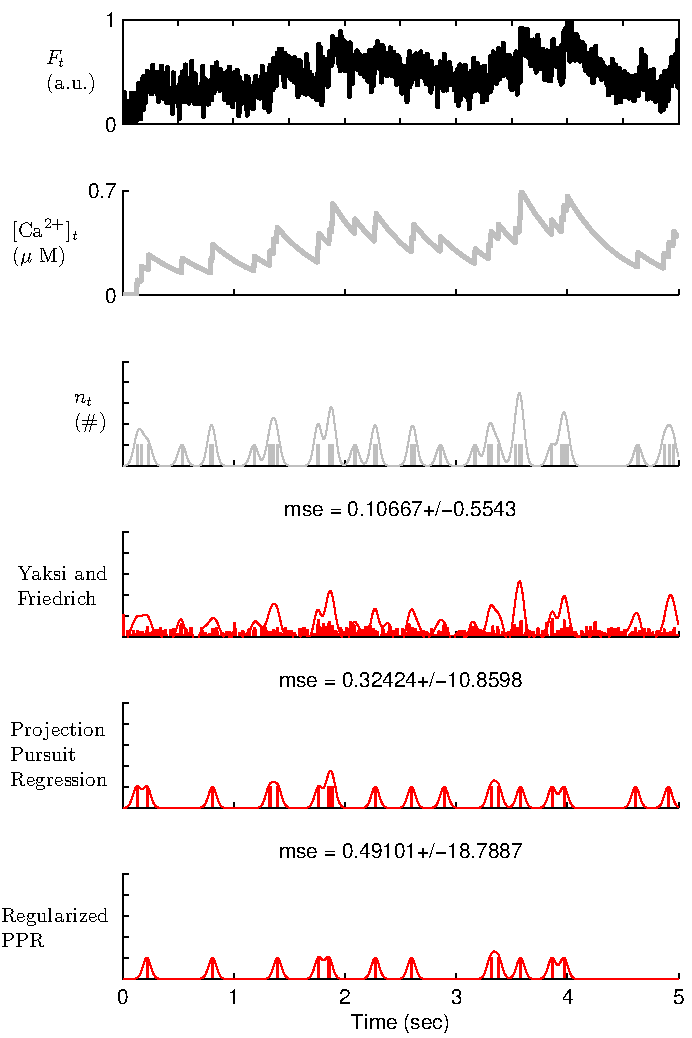
\includegraphics[width=1.0\linewidth]{comp1}
\caption{Comparison of various methods of inferring spike times. % (A) Observed fluorescence signal.  (B) True spike train.  (C) Naive inferred spike train using \eqref{eq:lsq}.  (D) Regularized spike train inference using \eqref{eq:reg}.  (E) Barrier method inferred spike train, using \eqref{eq:b}. (F) Projection pursuit regression inferred spike train, using \eqref{eq:ppr}.  All inferences used the same parameter values: $A=$ $\mu$M, $\tau=$ sec.
} \label{fig:comp}
\end{figure}

\begin{figure} \centering 
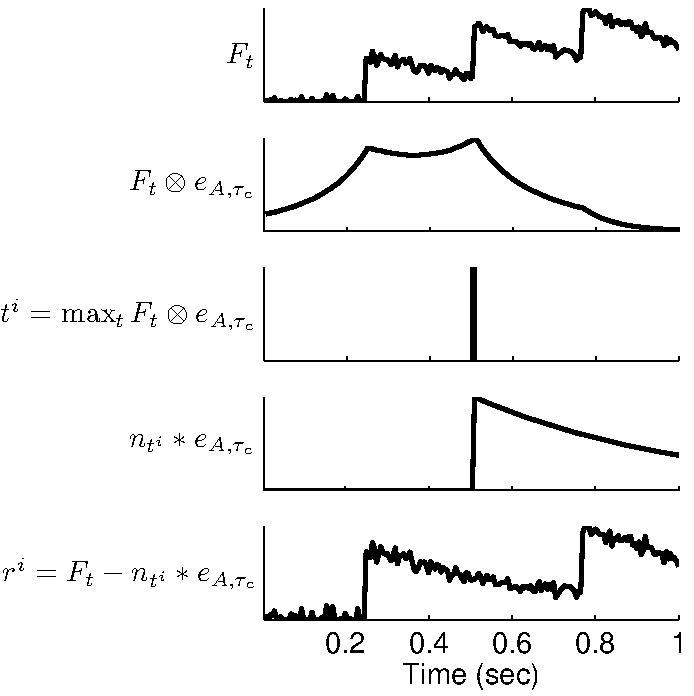
\includegraphics[height=0.8\textheight]{ppr_schem} 
\end{figure}


\newpage
\bibliography{C:/D/misc/biblist}
\addcontentsline{toc}{section}{References}
%\bibliographystyle{apalike}
\bibliographystyle{biophysj}



\end{document}
